\newpage
\section{OpenCV THRESH\_TRIANGLE }
Since the function THRESH\_TRIANGLE is not very well described in the OpenCV documentation here is a small explanation of it. First the function builds the histogram of the given image. Next it searches for the highest point and the first values from the border left and right which are not zero. Then it compares the distance between the position of the highest point and the position of the first non zero points left and right. The point with the bigger distance is used as an corner point for a triangle. The triangle can be seen in the figure\ref{theory:triangle}.

\begin{figure}[ht]
	\centering
	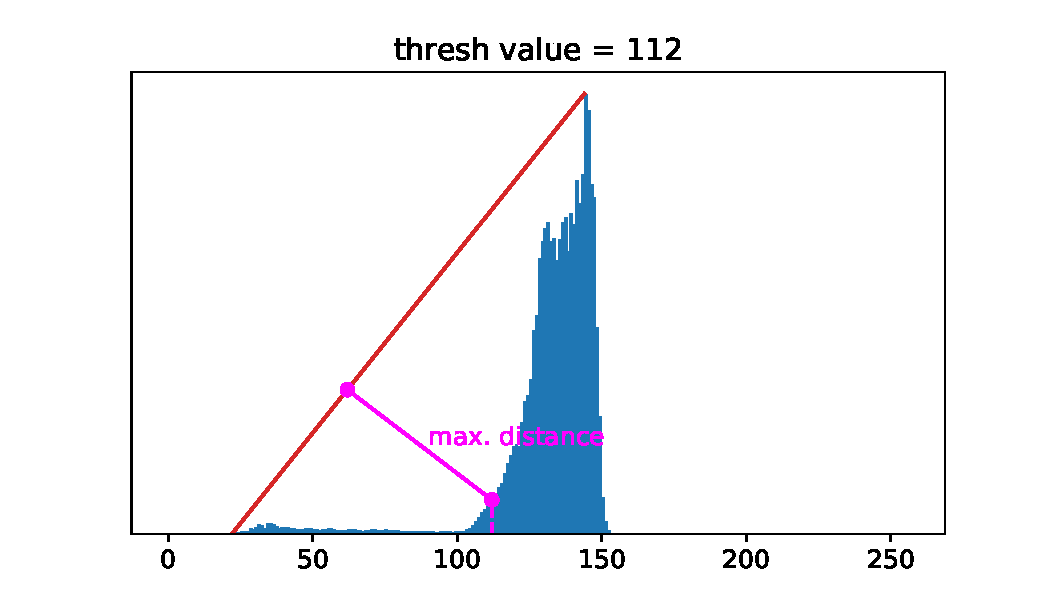
\includegraphics[width=\textwidth]{2-theory/threshold/triangle.pdf}
	\caption{Threshold triangle shown in histogram\label{theory:triangle}}
\end{figure} 
The hypotenuse of the triangle is now used to find orthogonal line between the hypotenuse and the histogram. To find this usually all values have to be calculated. But to find the correct length between the histogram and there is some complex geometry involved which is time consuming. To make the algorithm faster OpenCV makes a approximation. To better understand what is calculated we look at the OpenCV C++ code\ref{theory:code} which implements the triangle threshold. 

\definecolor{codegreen}{rgb}{0,0.6,0}
\definecolor{codegray}{rgb}{0.5,0.5,0.5}
\definecolor{codepurple}{rgb}{0.8,0,0.82}
\definecolor{backcolour}{rgb}{0.95,0.95,0.92}
\definecolor{dred}{rgb}{0.7,0,0}

\lstdefinestyle{mystyle}{
	backgroundcolor=\color{backcolour},   
	commentstyle=\color{codegreen},
	keywordstyle=\color{dred},
	numberstyle=\tiny\color{codegray},
	stringstyle=\color{codepurple},
	basicstyle=\footnotesize,
	breakatwhitespace=false,         
	breaklines=true,                 
	captionpos=b,                    
	keepspaces=true,                 
	numbers=left,                    
	numbersep=2pt,                  
	showspaces=false,                
	showstringspaces=false,
	showtabs=false,                  
	tabsize=2
}
\lstset{style=mystyle}
\lstdefinestyle{mystyle}{
	morekeywords={cwt,contourf,datetick}
} 


\begin{figure}[ht]
	\centering
	\lstinputlisting[language=C++,firstline=1301,lastline=1310,numbers=left,style = mystyle]{2-theory/threshold/thresh.cpp}
	\caption{OpenCV C++ code snipped}
	\label{theory:code}
\end{figure}
In the line one we have our max height a and the distance between left border and the place where a is located. The histogram is saved in the array h with 256 places, where the place itself represents the brightness value from zero to 255.
\newpage